\subsection{W+Jets MC Modelling Validation from CR1}
\label{sec:cr1}


The estimate of the uncertainty on this background is based on CR1, 
defined by applying the full signal selection, including the isolated track veto, but requiring 0 b-tags
(CSV medium working point as described in Sec.~\ref{sec:selection}). 
The sample is dominanted by \wjets\ and is thus used to validate the MC modelling of this background. 

In Table~\ref{tab:cr1mtsf} we show the amount that we need to scale the Wjets MC
by in order to have agreement between data and Monte Carlo in the $M_T$ peak 
region, defined as $60 < M_T < 100$ GeV.  These scale factors are not terribly 
important, but it is reassuring that they are not too different from 1.  (ARE THESE
SCALED FOR TRIGGER EFFICIENCY???)


\begin{table}[!h]
\begin{center}
\begin{tabular}{l||c||c|c|c|c}
\hline
Sample              & CR1PRESEL & CR1A & CR1B & CR1C & CR1D \\
\hline
\hline
Muon \mt-SF       & $0.91 \pm 0.03$ & $0.96 \pm 0.07$ & $0.88 \pm 0.11$ & $1.05 \pm 0.21$ & $1.27 \pm 0.41$ \\
\hline
\hline
Electron \mt-SF           & $0.82 \pm 0.03$ & $0.86 \pm 0.06$ & $1.09 \pm 0.15$ & $1.24 \pm 0.30$ & $1.11 \pm 0.40$ \\
\hline
\end{tabular}
\caption{ \mt\ peak Data/MC scale factors applied to the single lepton
  samples and \ttdl. The raw MC is used for backgrounds from rare
  processes. CR1PRESEL refers to a sample with $\met>50$ GeV.
  The uncertainties are statistical only.
\label{tab:cr1mtsf}}
\end{center}
\end{table}


In Table~\ref{tab:cr1yields} we compare the data and MC yields in the four $M_T$ signal regions
and in a looser control region.  We also derive the data/MC scale factors 
$SFR^{e}_{wjet}$ and  $SFR^{\mu}_{wjet}$.  The underlying \met\ and $M_T$ distributions
are shown in Fig.~\ref{fig:cr1met}  and~\ref{fig:cr1mtrest}

\begin{table}[!h]
\begin{center}
\begin{tabular}{l||c||c|c|c|c}
\hline
Sample              & CR1PRESEL & CR1A & CR1B & CR1C & CR1D \\
\hline
\hline
Muon MC                   & $456 \pm 73$ & $174 \pm 44$ & $51 \pm 7$ & $18 \pm 2$ & $10 \pm 2$ \\
Muon Data                 & $657$ & $246$ & $142$ & $43$ & $12$ \\
\hline
Muon Data/MC SF:  ($SFR^{\mu}_{wjet}$)        & $1.44 \pm 0.24$ & $1.41 \pm 0.37$ & $2.80 \pm 0.47$ & $2.37 \pm 0.46$ & $1.23 \pm 0.42$ \\
\hline
\hline
Electron MC               & $396 \pm 64$ & $147 \pm 36$ & $54 \pm 4$ & $19 \pm 2$ & $8 \pm 2$ \\
Electron Data             & $702$ & $223$ & $144$ & $50$ & $23$ \\
\hline
Electron Data/MC SF:  ($SFR^e_{wjet}$)   & $1.77 \pm 0.29$ & $1.52 \pm 0.39$ & $2.68 \pm 0.30$ & $2.57 \pm 0.49$ & $2.73 \pm 0.76$ \\
\hline
\end{tabular}
\caption{ Yields in \mt\ tail comparing the MC prediction (after
  applying SFs) to data. CR1PRESEL refers to a sample with $\met>50$
  GeV and $\mt>150$ GeV.
  The uncertainties are statistical only. VERENA MAKE SURE YOU ADD SCALE FACTOR SYMBOLS TO THIS TABLE.
\label{tab:cr1yields}}
\end{center}
\end{table}


\begin{figure}[hbt]
  \begin{center}
        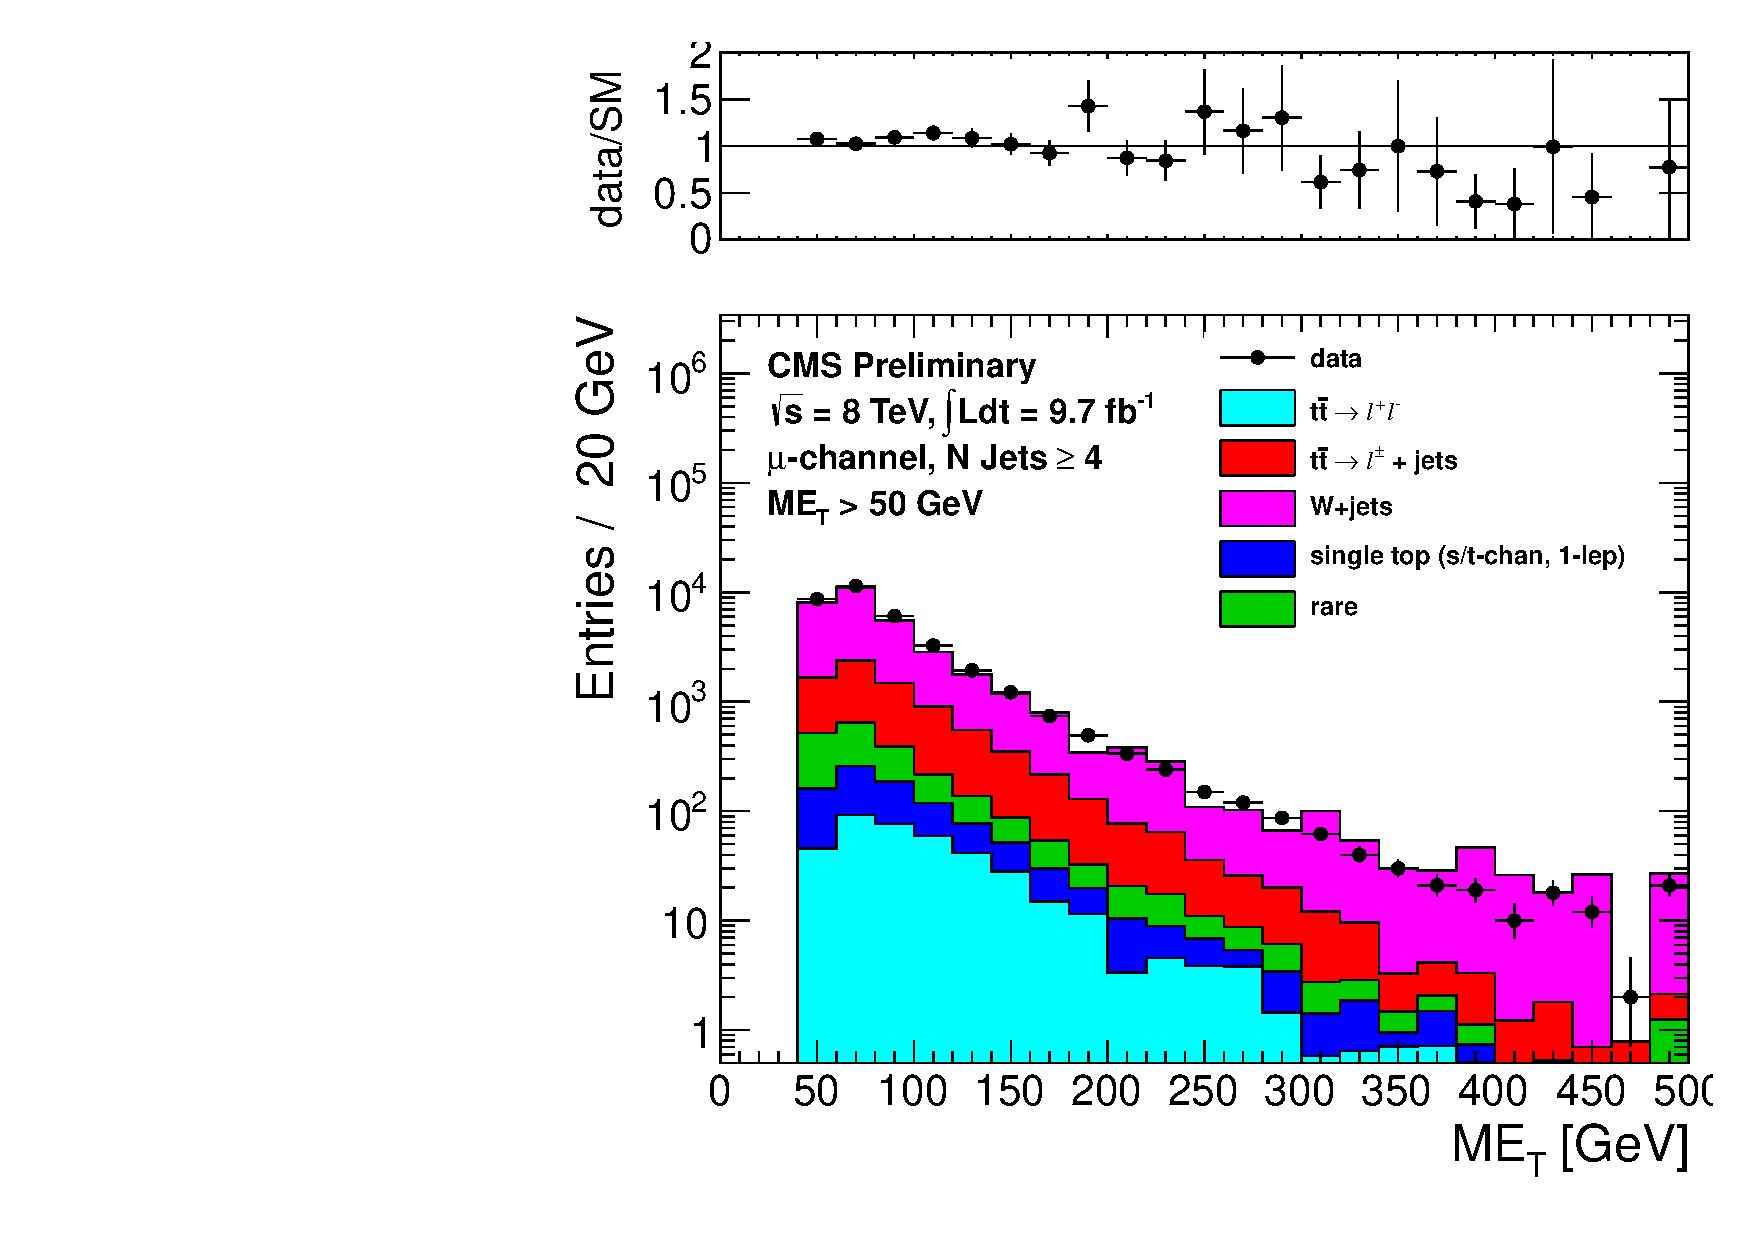
\includegraphics[width=0.5\linewidth]{plots/CR1plots/met_met50_leadmuo_nj4.pdf}%
        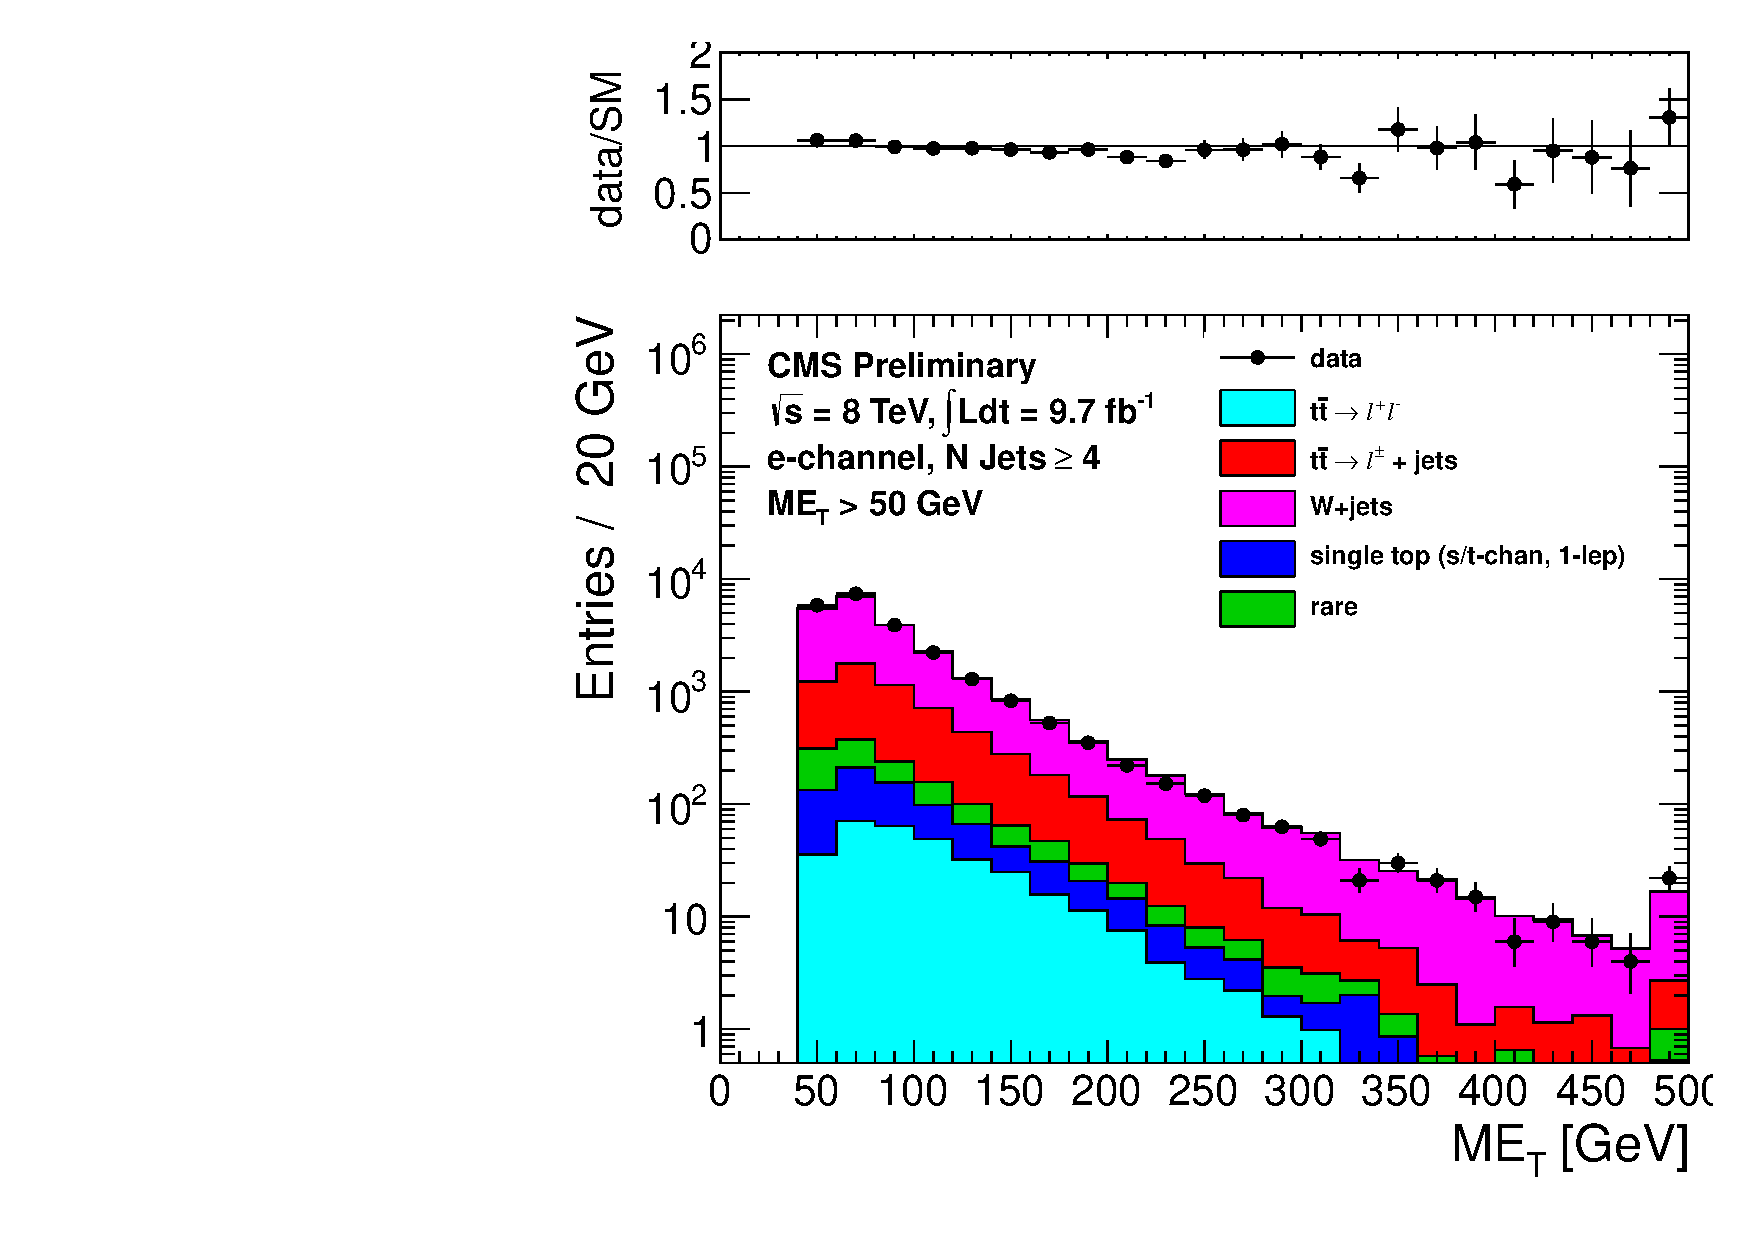
\includegraphics[width=0.5\linewidth]{plots/CR1plots/met_met50_leadele_nj4.pdf}
        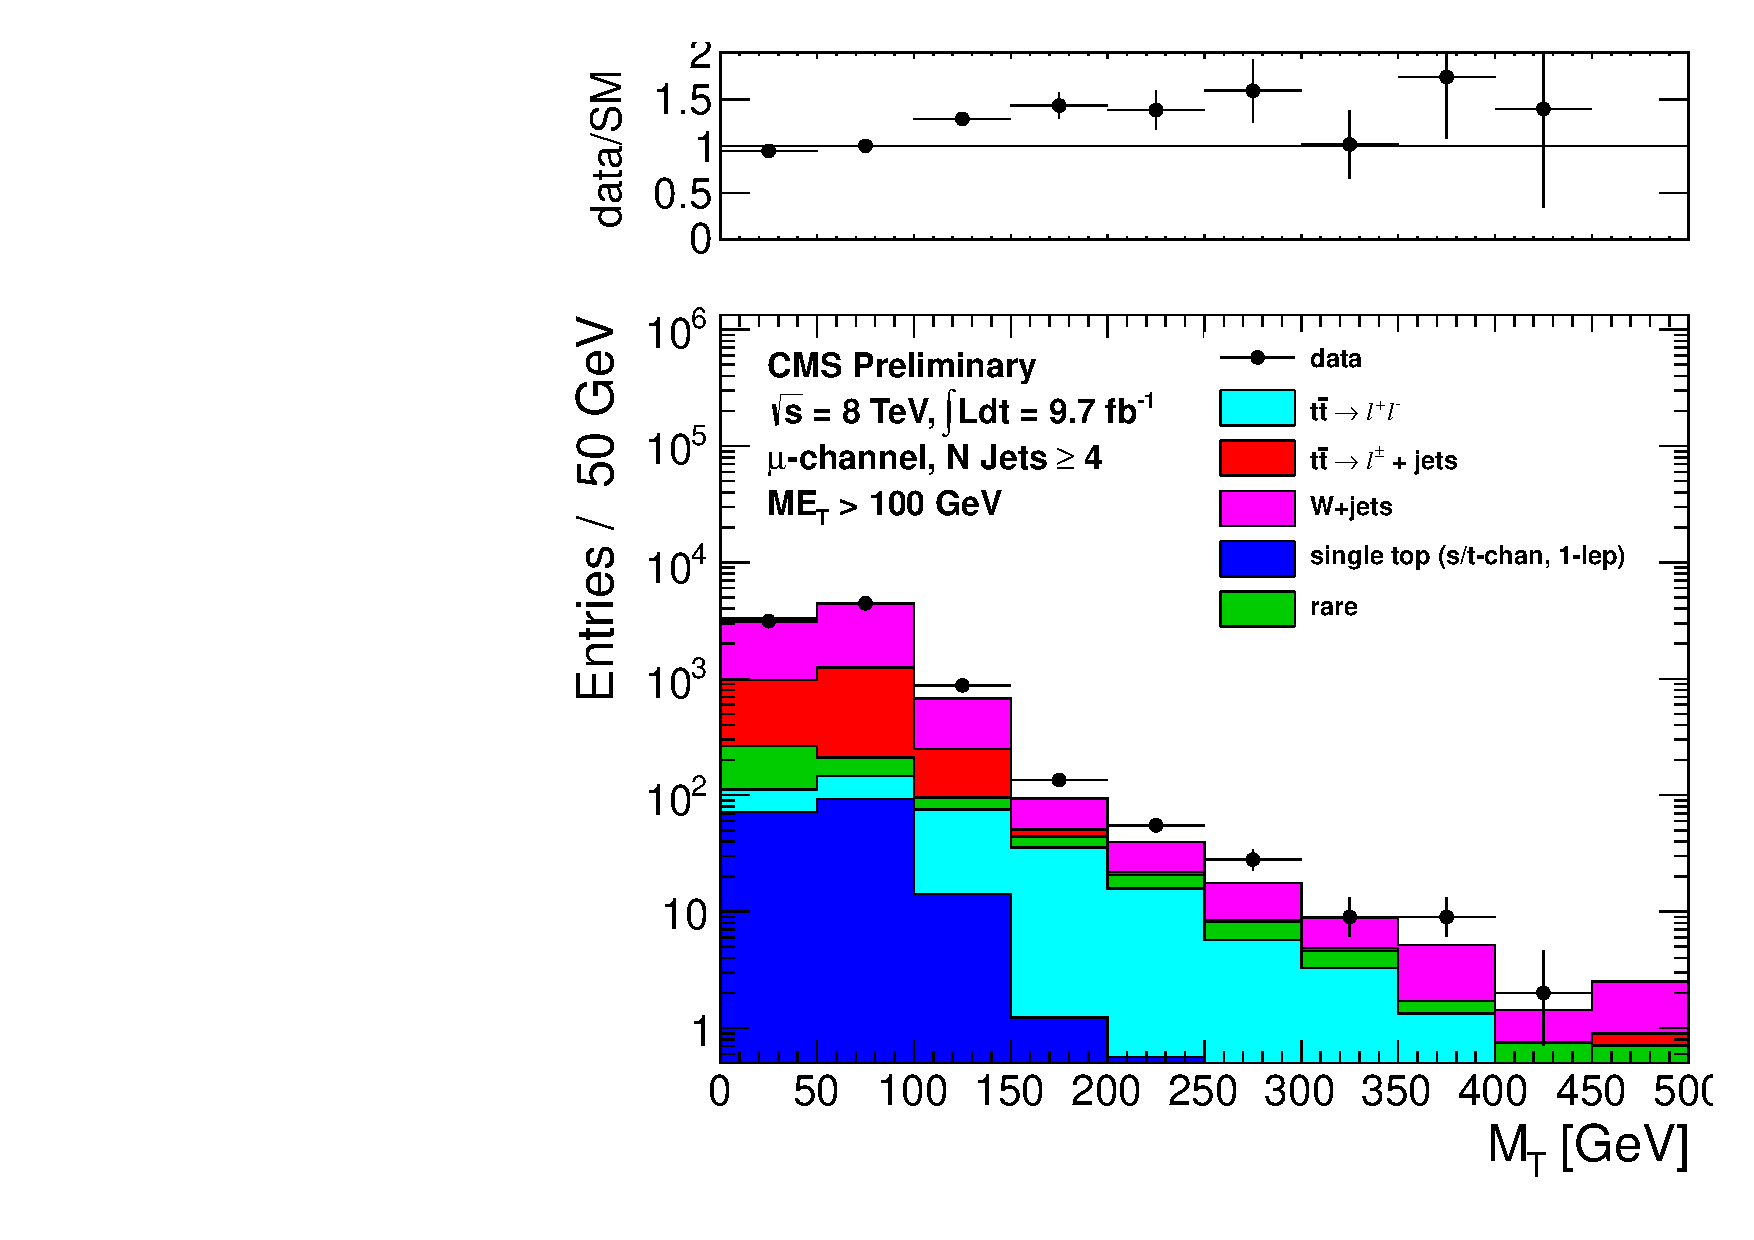
\includegraphics[width=0.5\linewidth]{plots/CR1plots/mt_met100_leadmuo_nj4.pdf}%
        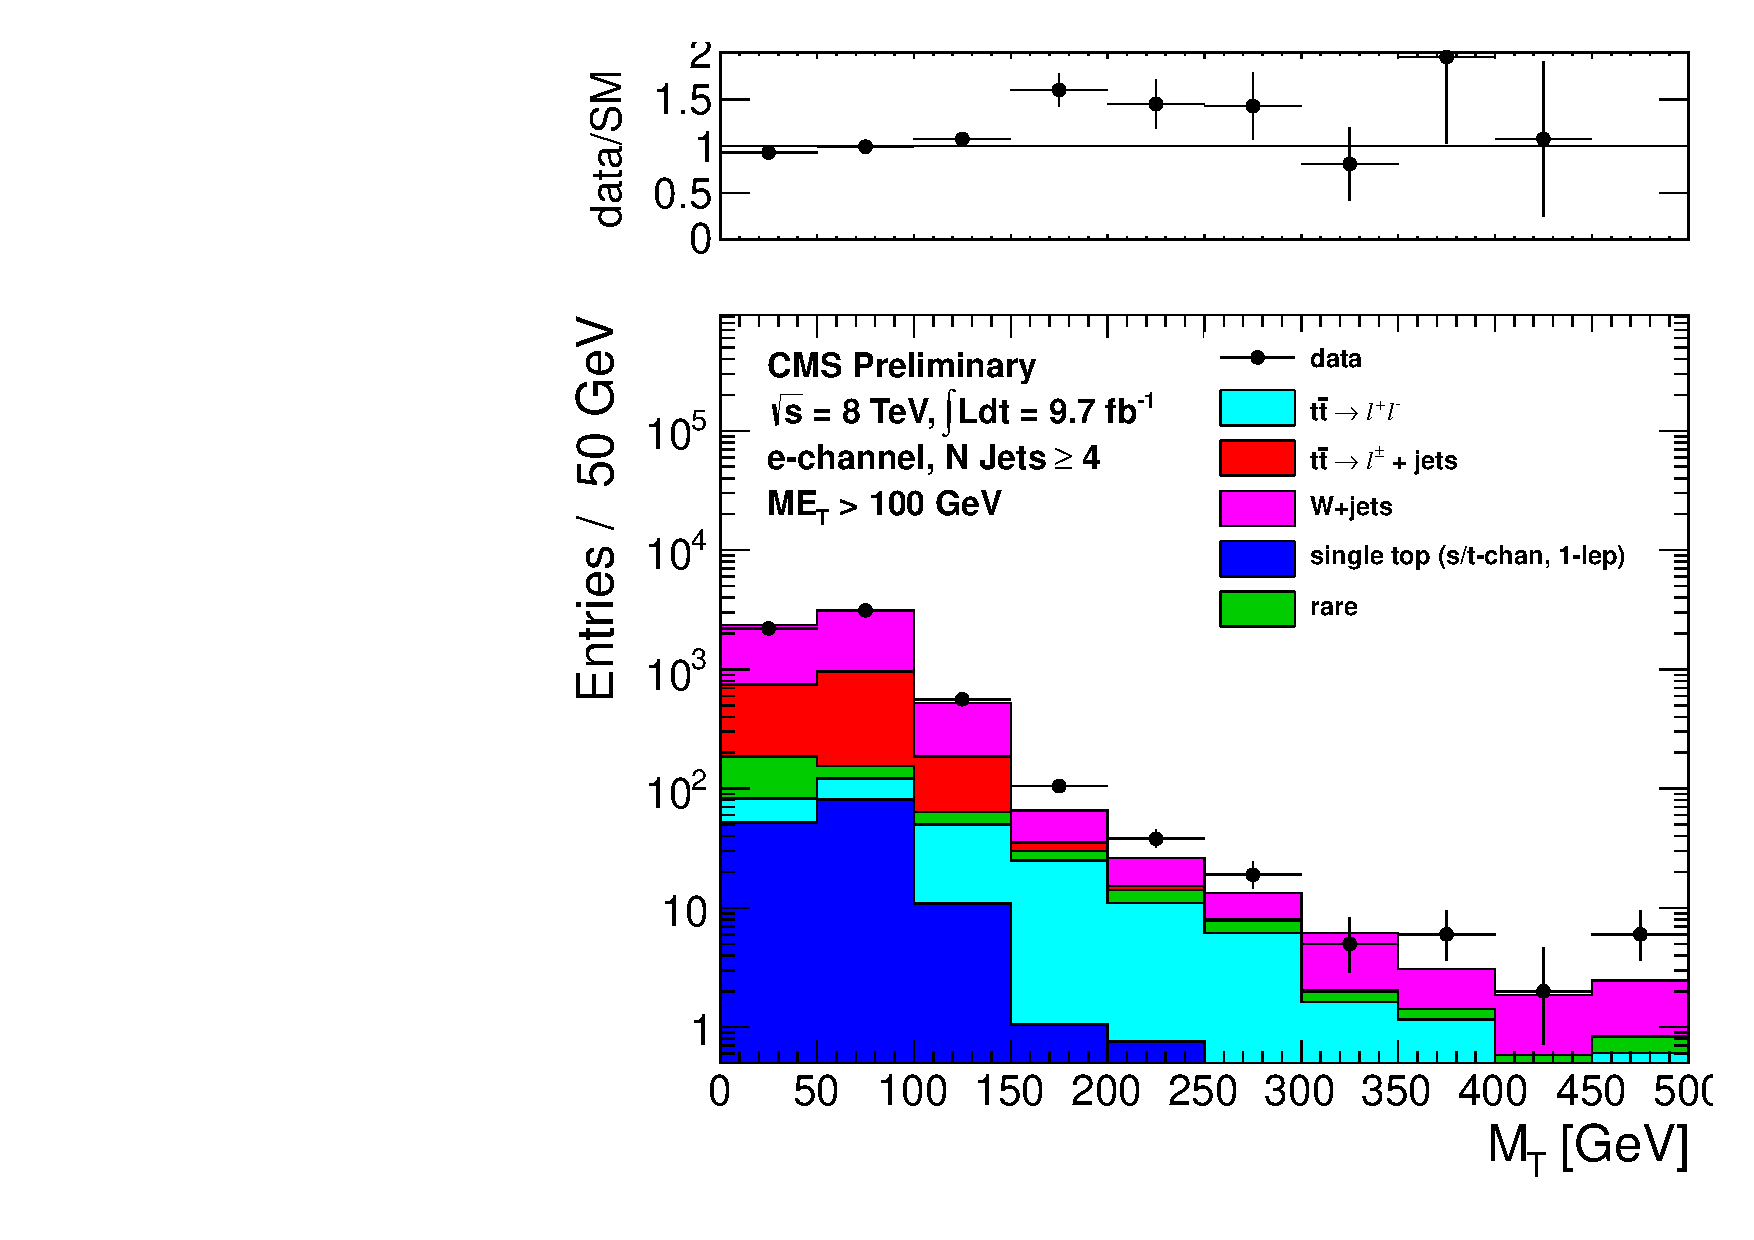
\includegraphics[width=0.5\linewidth]{plots/CR1plots/mt_met100_leadele_nj4.pdf}
    \caption{
      Comparison of the \met\ (top) and \mt\ for $\met>100$ (bottom) distributions in data vs. MC for events
      with a leading muon (left) and leading electron (right)
      satisfying the requirements of CR1. 
\label{fig:cr1met} 
}  
      \end{center}
\end{figure}


\begin{figure}[hbt]
  \begin{center}
        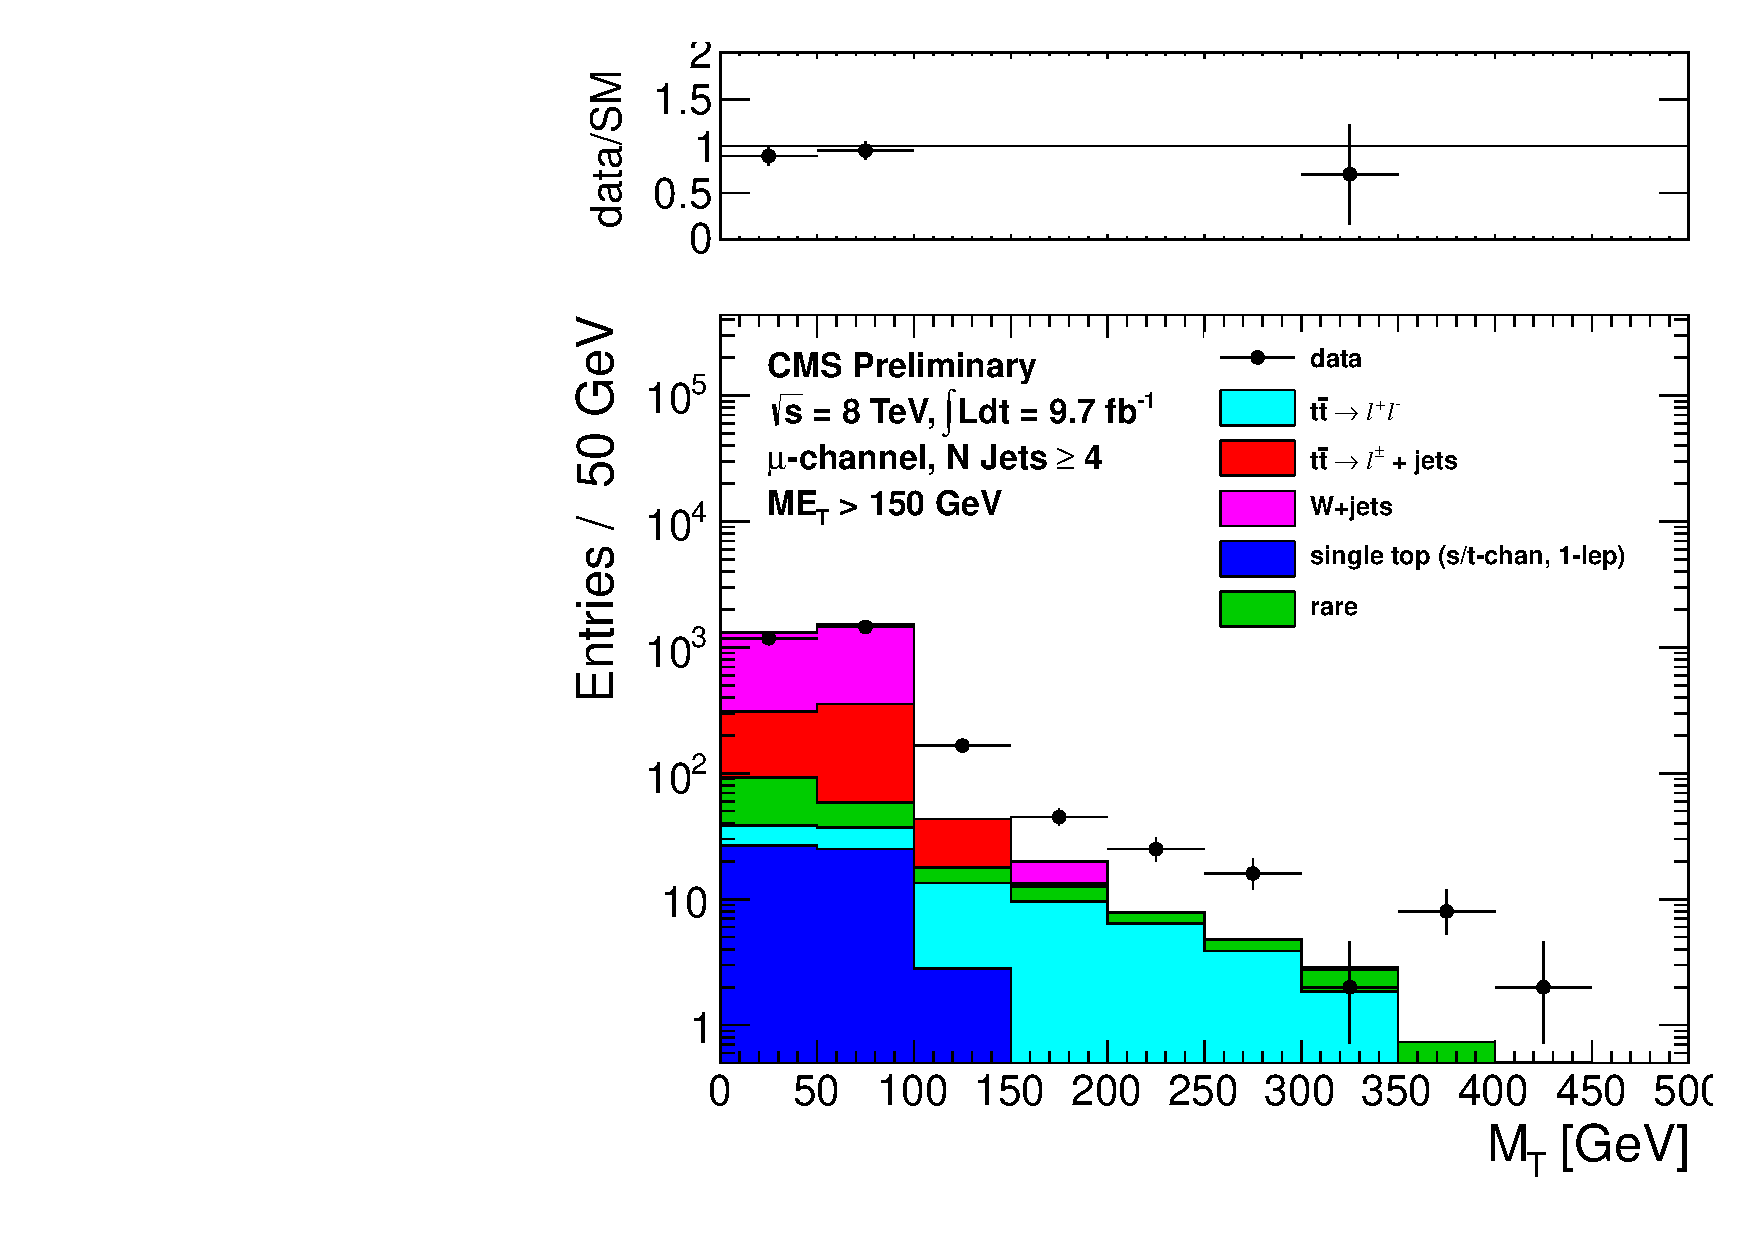
\includegraphics[width=0.5\linewidth]{plots/CR1plots/mt_met150_leadmuo_nj4.pdf}%
        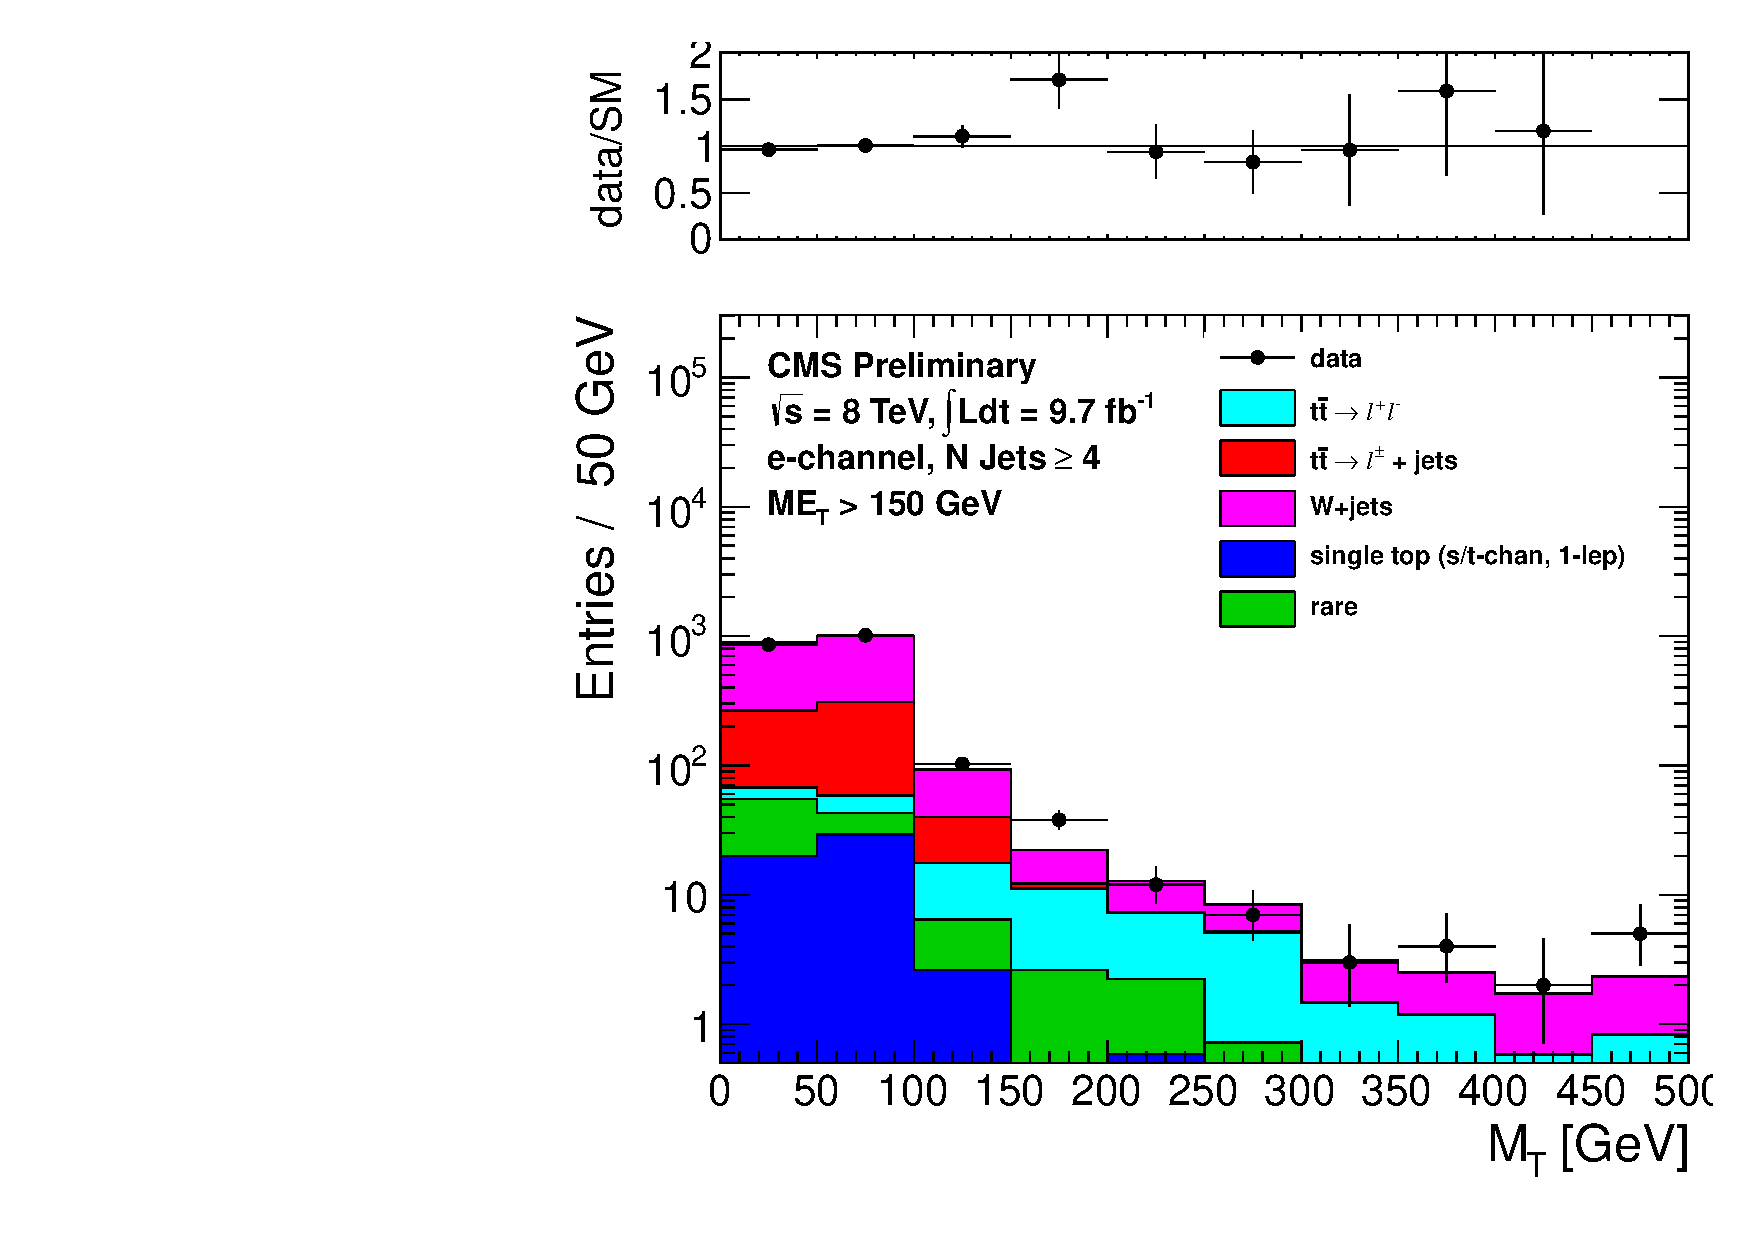
\includegraphics[width=0.5\linewidth]{plots/CR1plots/mt_met150_leadele_nj4.pdf}
        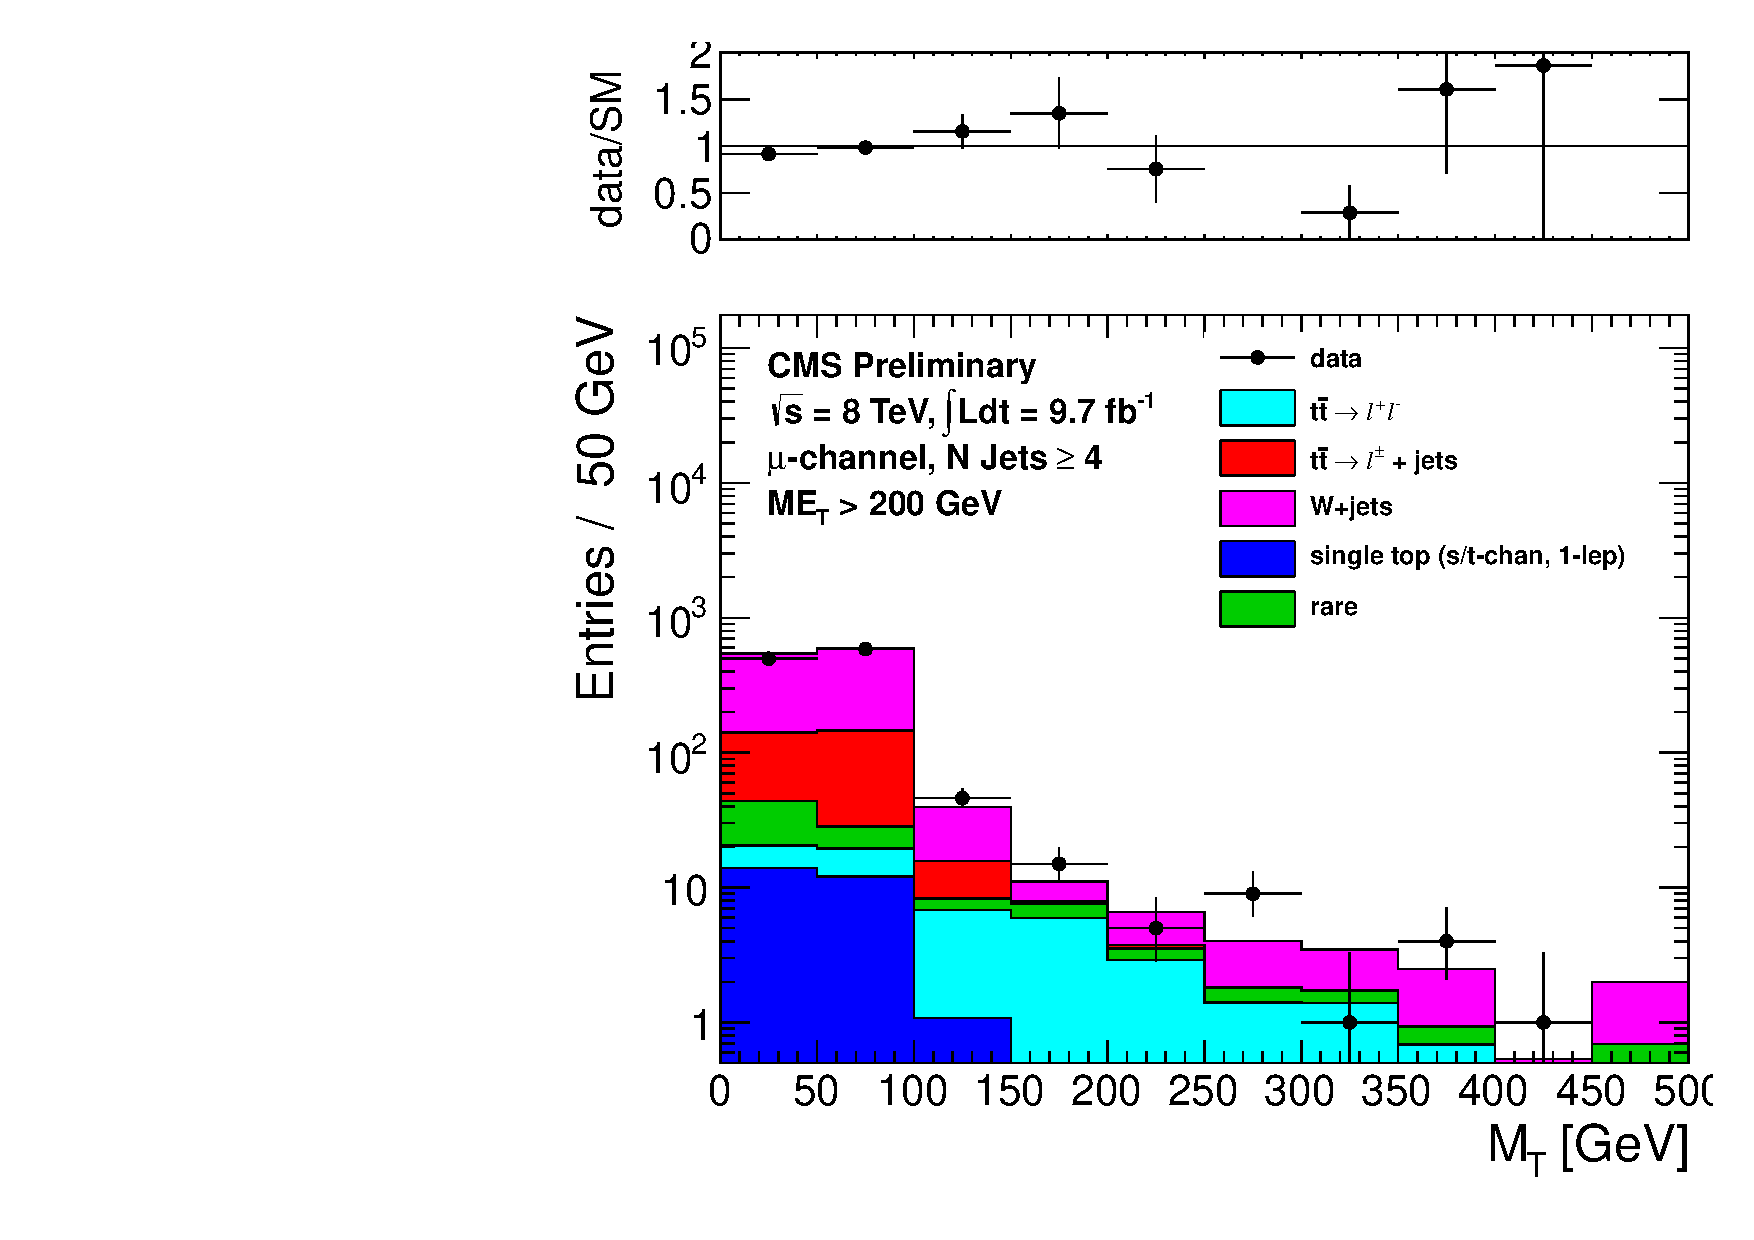
\includegraphics[width=0.5\linewidth]{plots/CR1plots/mt_met200_leadmuo_nj4.pdf}%
        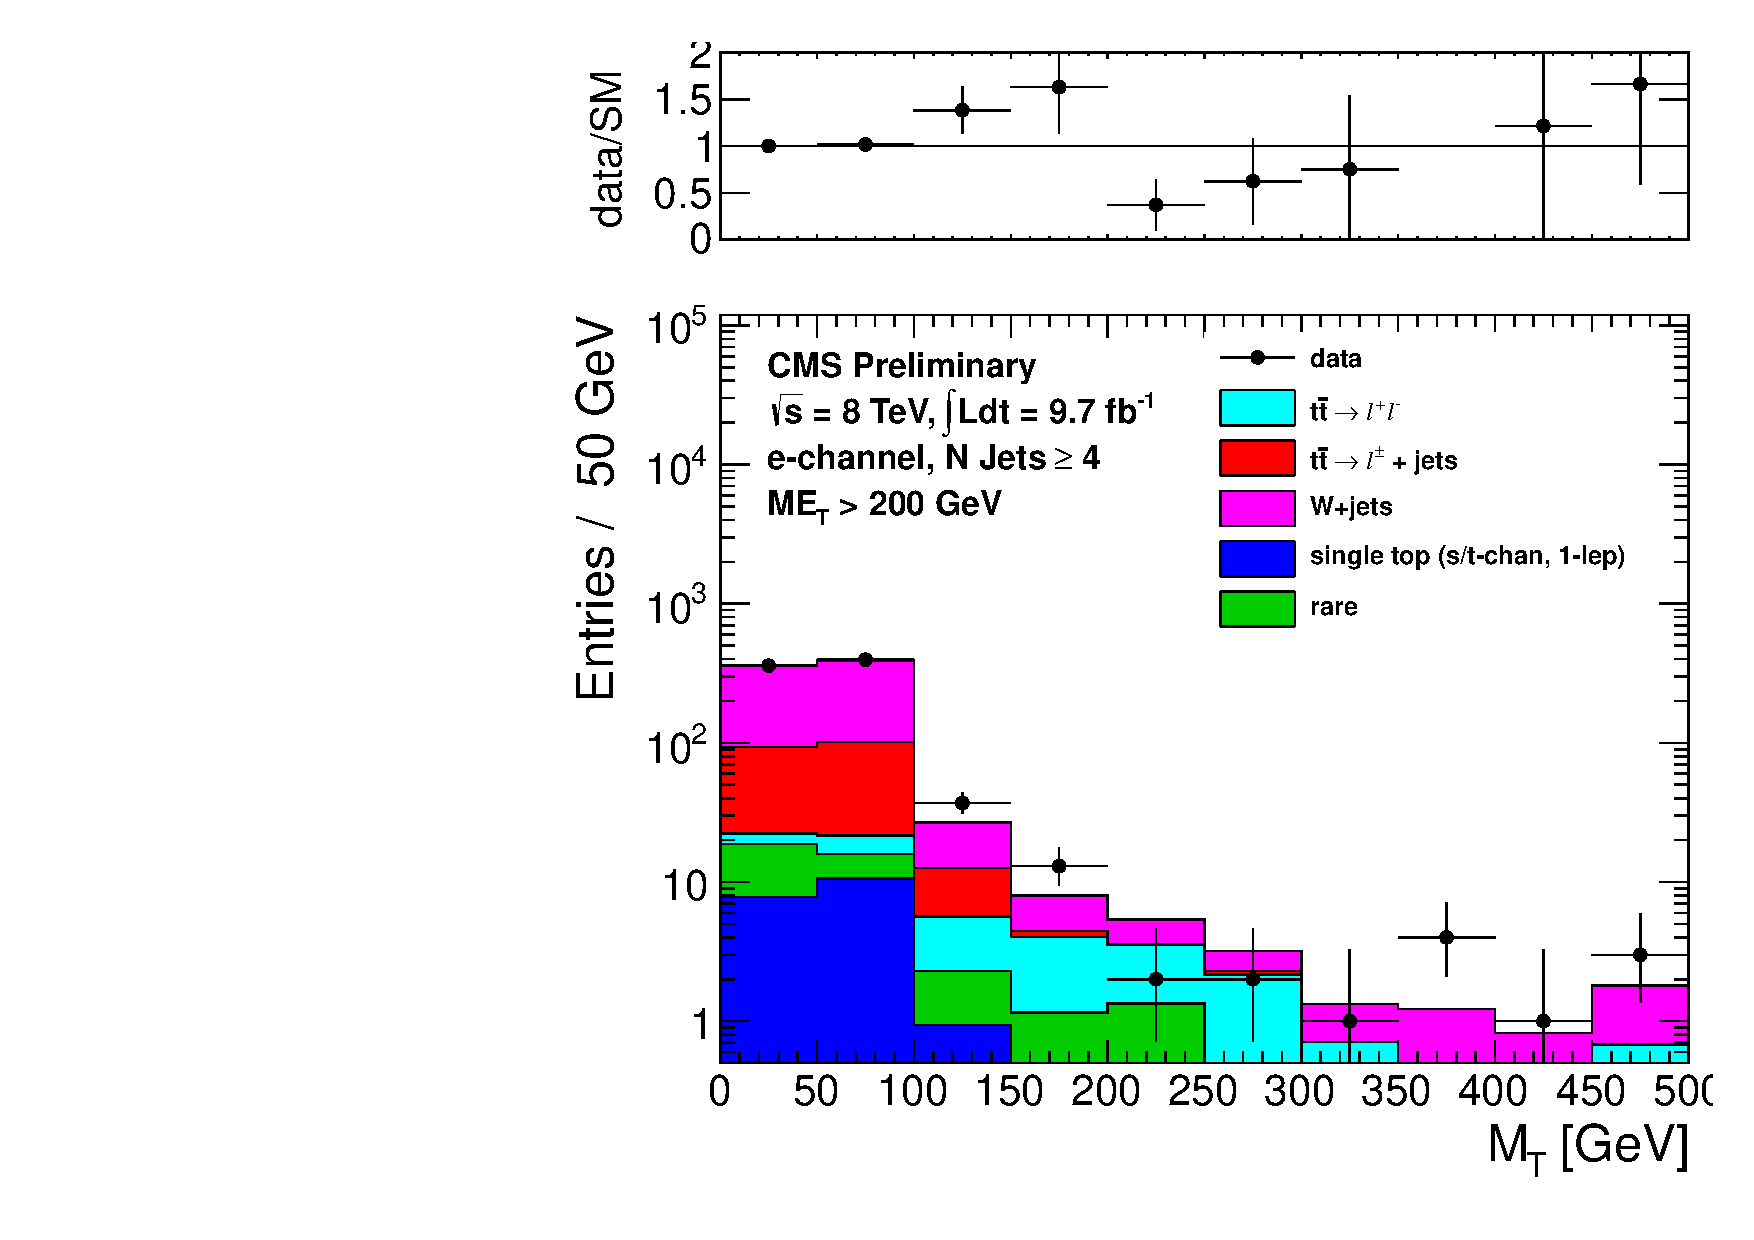
\includegraphics[width=0.5\linewidth]{plots/CR1plots/mt_met200_leadele_nj4.pdf}
        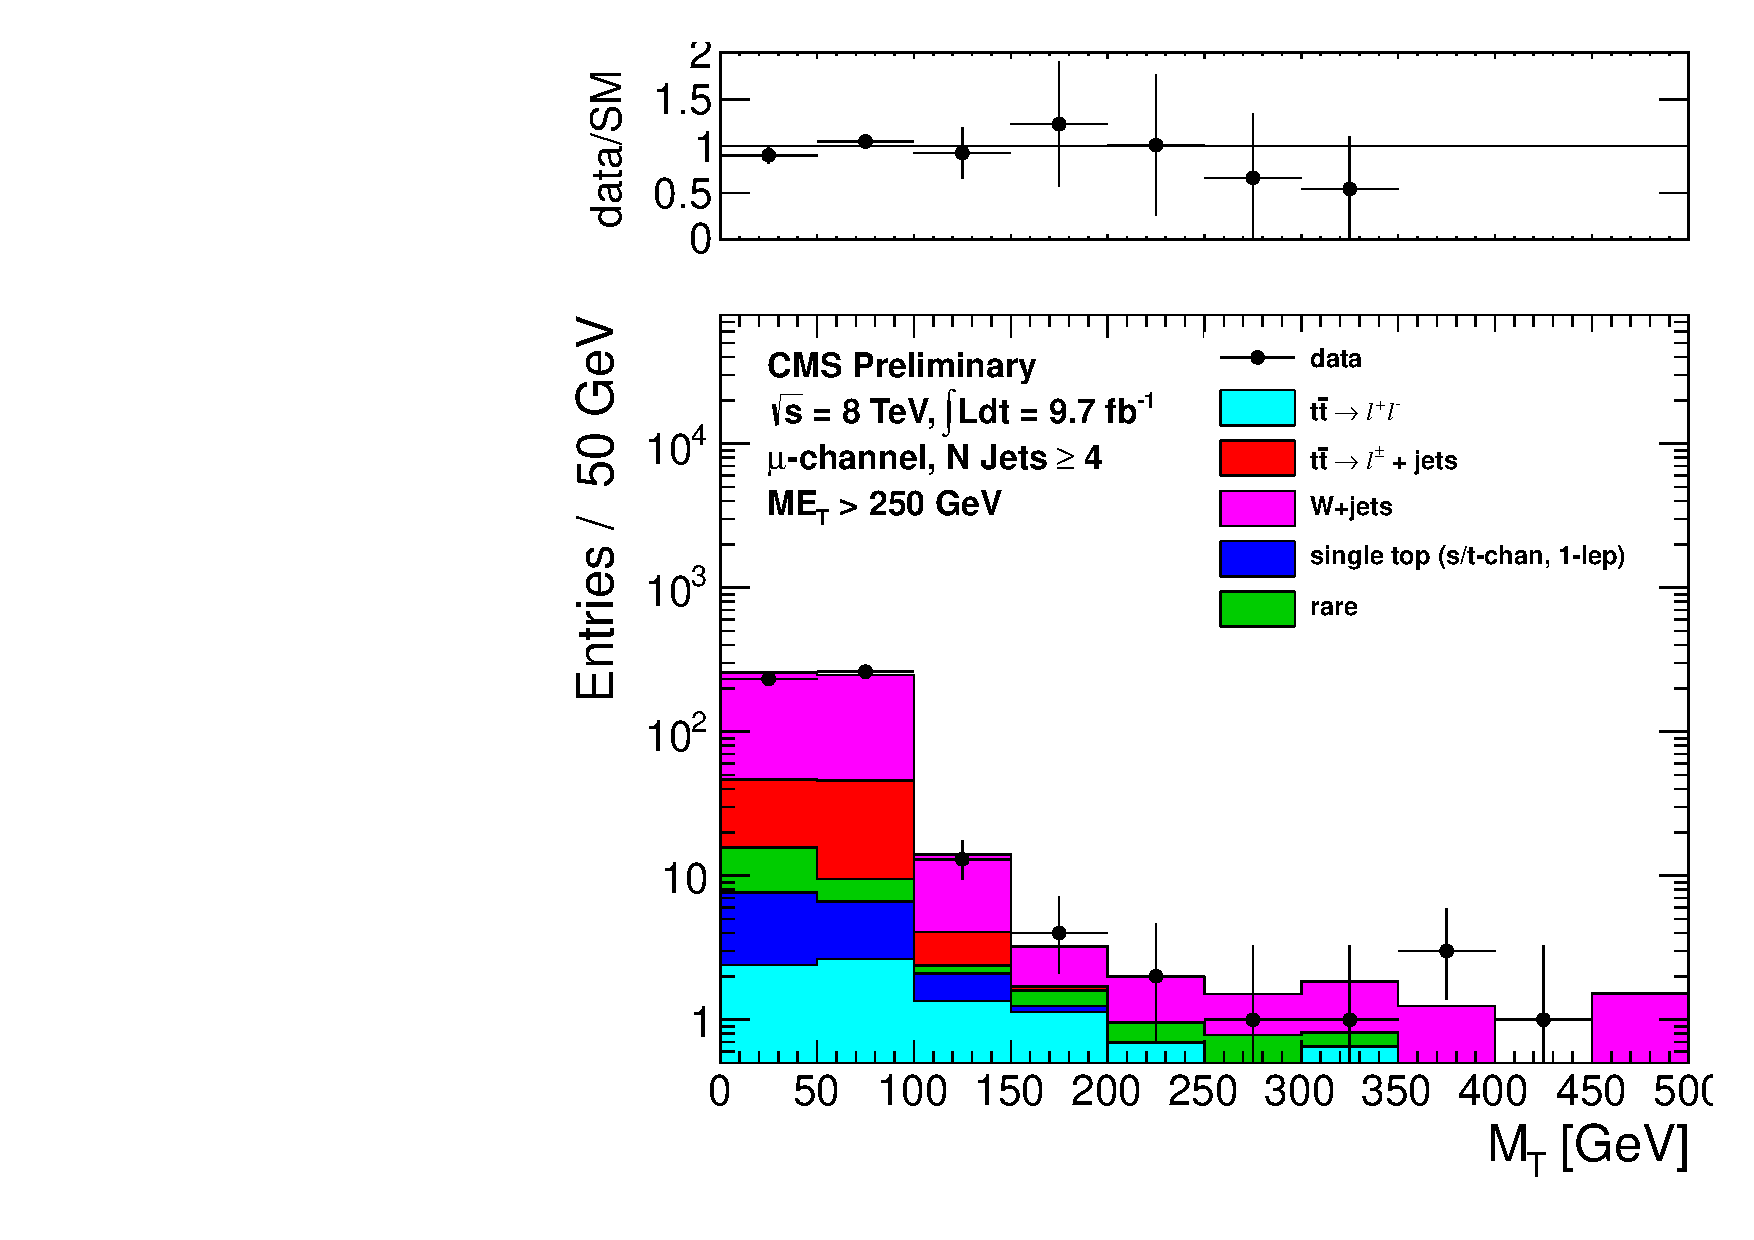
\includegraphics[width=0.5\linewidth]{plots/CR1plots/mt_met250_leadmuo_nj4.pdf}%
        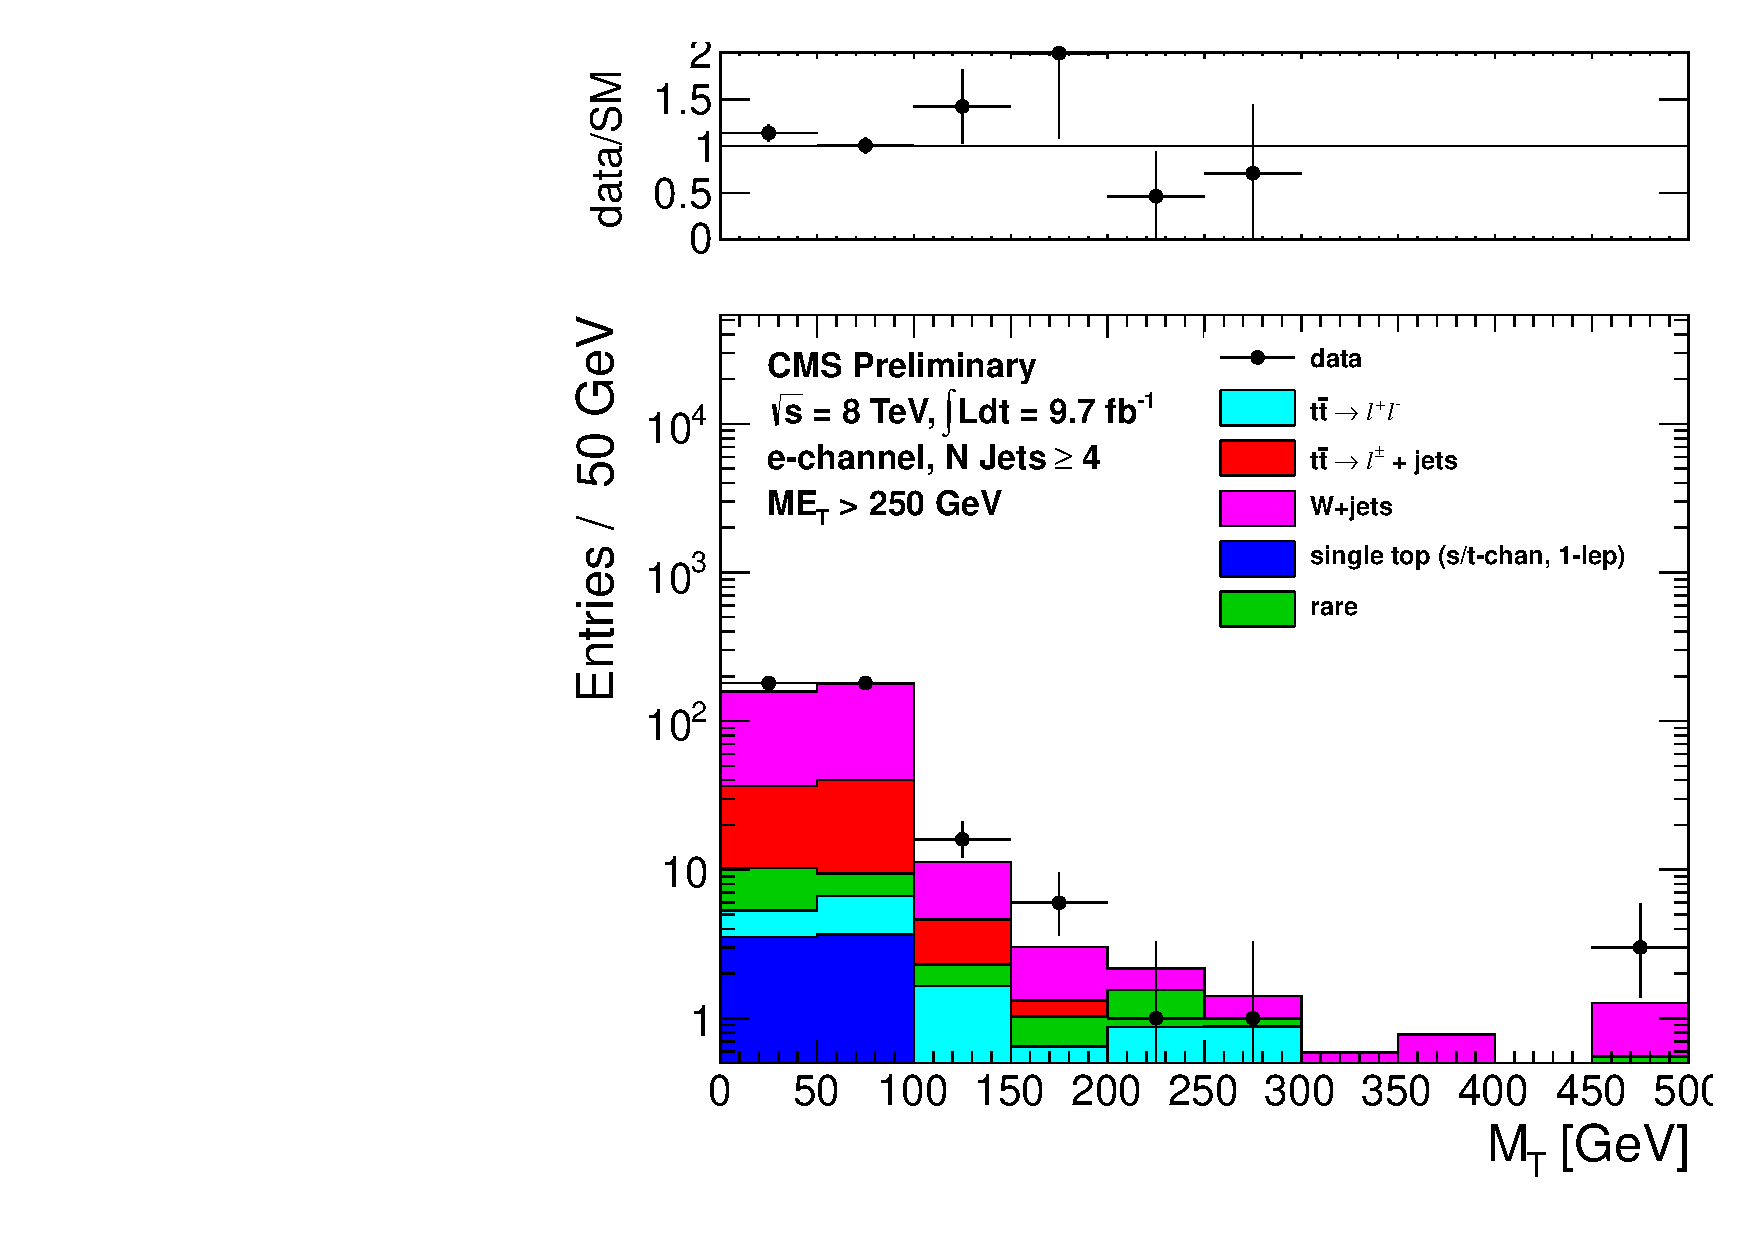
\includegraphics[width=0.5\linewidth]{plots/CR1plots/mt_met250_leadele_nj4.pdf}
    \caption{
      Comparison of the \mt\ distribution in data vs. MC for events
      with a leading muon (left) and leading electron (right)
      satisfying the requirements of CR1. The \met\ requirements used are
      150 GeV (top), 200 GeV (middle) and 250 GeV (bottom).
\label{fig:cr1mtrest} 
}  
      \end{center}
\end{figure}

\clearpage